\documentclass[../../../../main.tex]{subfiles}
\begin{document}

\begin{flushright}
\footnotesize\textit{【自動文字起こし・要確認】}
\end{flushright}

[解] $\alpha < \beta \dots$ ①として良い。$PQ^2 = PR^2$ だから、
\begin{align*}
(\beta - \frac{1}{2})^2 + (\beta^2 - \frac{1}{4})^2 &= (\alpha - \frac{1}{2})^2 + (\alpha^2 - \frac{1}{4})^2 \\
\beta^2 - \beta + \beta^4 - \frac{1}{2}\beta^2 &= \alpha^2 - \alpha + \alpha^4 - \frac{1}{2}\alpha^2 \\
\beta^4 + \frac{1}{2}\beta^2 - \beta &= \alpha^4 + \frac{1}{2}\alpha^2 - \alpha \\
(\beta^2 + \alpha^2)(\beta^2 - \alpha^2) + \frac{1}{2}(\beta^2 - \alpha^2) - (\beta - \alpha) &= 0
\end{align*}
$\alpha \neq \beta$ から
\[ (\beta^2 + \alpha^2)(\beta + \alpha) + \frac{1}{2}(\beta + \alpha) - 1 = 0 \quad \cdots \text{①} \]
ここで、$p = \alpha + \beta, \ q = \alpha \beta$ とすると、$\alpha, \beta$ の実数条件から、
\[ p^2 - 4q > 0 \quad \cdots \text{②} \]
である。①に代入して
\[ (p^2 - 2q)p + \frac{1}{2}p = 1 \quad \cdots \text{③} \]
次に、$G$ について
\begin{align*}
X &= \frac{\alpha+\beta+\frac{1}{2}}{3} = \frac{1}{3}(p+\frac{1}{2}) \quad \cdots * \\
Y &= \frac{\alpha^2+\beta^2+\frac{1}{4}}{3} = \frac{1}{3}(p^2-2q+\frac{1}{4})
\end{align*}
である。③において、$p=0$ とすると $0=1$ となり矛盾、つまり $p \neq 0 \dots$ ④ であるから
\[ q = \frac{1}{2} \left( p^2 - \frac{1}{p} + \frac{1}{2} \right) \]
となる。②、*に代入して、
\[ \begin{cases}
p^2 - 2 \left( \frac{1}{2}(p^2 - \frac{1}{p} + \frac{1}{2}) \right) > 0 \\
Y = \frac{1}{3} \left( p^2 - p^2 + \frac{1}{p} - \frac{1}{2} + \frac{1}{4} \right) = \frac{1}{3}(\frac{1}{p} - \frac{1}{4})
\end{cases} \]
\[ \begin{cases}
-p(p-1)(p^2+p+2) > 0 \\
X = \frac{1}{3}(p+\frac{1}{2}) \implies p = 3X - \frac{1}{2} \ (\text{※式展開の都合で } X = \frac{1}{3}(\frac{1}{p}-\frac{1}{4}) \text{ は下段の } Y \text{ の計算})
\end{cases} \]
（※原稿の記述： $Y = \frac{1}{3}(\frac{1}{p}-\frac{1}{4})$, $X = \frac{1}{3}(p+\frac{1}{2})$ ）
から、$p^2+p+2 = (p+\frac{1}{2})^2 + \frac{7}{4} > 0$ に注意して $0 < p < 1$ である。*から $p = 3X - \frac{1}{2}$ だから、
\[ \begin{cases}
0 < 3X - \frac{1}{2} < 1 \\
Y = \frac{1}{3} \left( \frac{1}{3X-\frac{1}{2}} - \frac{1}{4} \right)
\end{cases} \]
\[ \begin{cases}
\frac{1}{6} < X < \frac{1}{2} \\
Y = \frac{1}{3} \left( \frac{2}{6X-1} - \frac{1}{4} \right)
\end{cases} \]

\begin{center}
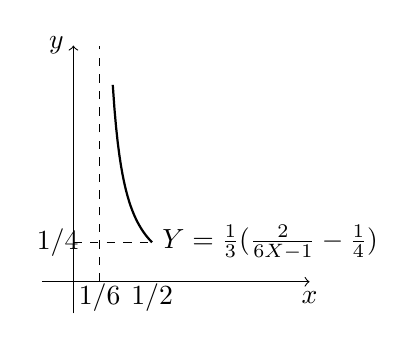
\begin{tikzpicture}[scale=2]
\draw[->] (-0.2, 0) -- (1.5, 0) node[below] {$x$};
\draw[->] (0, -0.2) -- (0, 1.5) node[left] {$y$};
\draw[domain=0.25:0.5, thick] plot (\x, {1/3*(2/(6*\x-1) - 1/4)}) node[right] {$Y = \frac{1}{3}(\frac{2}{6X-1} - \frac{1}{4})$};
\draw[dashed] (1/6, 0) -- (1/6, 1.5);
\node at (1/6, -0.1) {$1/6$};
\node at (1/2, -0.1) {$1/2$};
\draw[dashed] (0, 1/4) -- (1/2, 1/4);
\node at (-0.1, 1/4) {$1/4$};
\end{tikzpicture}
\end{center}

\end{document}
